\documentclass[conference]{IEEEtran}
% \IEEEoverridecommandlockouts
% The preceding line is only needed to identify funding in the first footnote. If that is unneeded, please comment it out.
\usepackage{cite}
\usepackage{amsmath,amssymb,amsfonts}
\usepackage{algorithmic}
\usepackage{graphicx}
\usepackage{float}
\usepackage{textcomp}
\usepackage{xcolor}
\usepackage{hyperref}
\def\BibTeX{{\rm B\kern-.05em{\sc i\kern-.025em b}\kern-.08em
    T\kern-.1667em\lower.7ex\hbox{E}\kern-.125emX}}

% GitHub link
\newcommand{\githublink}{\url{https://github.com/himangg/Cuisine-Recommendation-System}}

\begin{document}

\title{Cuisine Recommendation System}

\author{\IEEEauthorblockN{1\textsuperscript{st} Himang Chandra Garg}
\IEEEauthorblockA{\textit{Computer Science and Engineering} \\
\textit{Indraprastha Institute of Information Technology}\\
Roll no.- 2022214 \\
himang22214@iiitd.ac.in}
\and
\IEEEauthorblockN{2\textsuperscript{nd} Nishil Agarwal}
\IEEEauthorblockA{\textit{Computer Science and Artificial Intelligence} \\
\textit{Indraprastha Institute of Information Technology}\\
Roll no.- 2022334 \\
nishil22334@iiitd.ac.in}
}

\maketitle

\begin{abstract}
 In this report, we present the design and implementation of a cuisine recommendation system aimed at assisting users in discovering recipes that align with their tastes and dietary requirements. Leveraging machine learning techniques such as content-based and collaborative filtering, our system analyzes user preferences, ingredient profiles, and historical interactions to generate personalized recipe suggestions.
\end{abstract}

% GitHub link
\section{GitHub Repository}
The source code for our project can be found at: \githublink

\section{Dataset}
% Details about the dataset used
For our project, we utilize a comprehensive dataset from Kaggle, comprising a diverse collection of Food recipes showcasing various regional cuisines and culinary traditions. The dataset includes essential information such as recipe names, ingredients, preparation time, nutritional content, and user ratings. In the earlier deadline we stated that we will be using.
https://www.kaggle.com/datasets/kritirathi/indian-food-dataset-with/data
but due to less rows we have changed our dataset to https://www.kaggle.com/datasets/irkaal/foodcom-recipes-and-reviews.

\section{Data Preprocessing}

In this section, we detail the preprocessing steps applied to the recipe dataset to prepare it for further analysis and modeling.

\subsection{Reading and Filtering Dataset}

The recipe dataset is initially read using the Pandas library, loading it into a DataFrame named \texttt{data}. Subsequently, irrelevant columns are filtered out to focus on essential attributes relevant to the recommendation system to reduce noise prevent unnecessary complexity.

\subsection{Removing Unnecessary Rows and Columns}

To enhance data consistency, we removed entries with missing ratings, incorrect/erroneous data etc. using the \texttt{drop} function.

\subsection{Selecting Diverse Rating Dishes}

Further, we stratified the dataset based on aggregated ratings, selecting a balanced mix of highly rated and lower-rated recipes for model training.

\subsection{Modifying Column Formats, Handling Missing and Erroneous Data}

 Additionally, we brought the entries of date\_of\_publication, cooking\_time, ingredients  columns into the required format for efficient handling of data. We also handled missing values in various columns, ensuring consistency and completeness.

\subsection{Removing Duplicate Entries}

Duplicate recipe names are removed from the dataset, ensuring uniqueness and avoiding redundancy in recommendations.

\subsection{Merging Datasets}

The preprocessed recipe dataset is merged with the reviews dataset based on \texttt{RecipeId}, facilitating the integration of user ratings into the recommendation system.

\subsection{Filtering Reviews}

Reviews from reviewers with less than five reviews are removed from the dataset, ensuring that only substantial reviews are considered in the analysis.

\subsection{Saving Processed Data}

The final preprocessed dataset is saved to a new file for further analysis and modeling.

\section{Data Visualization}

In this section, we present visualizations of various aspects of the processed dataset to gain insights into recipe categories, rating distribution, publication trends, calorie distribution, and top recipes and authors based on review count.

\subsection{Distribution of Recipe Categories}

The distribution of recipe categories is visualized using a pie chart. Rare categories, representing less than 1 percent of the dataset, are grouped under 'Others' to simplify the visualization.

\begin{figure}[H]
\centering
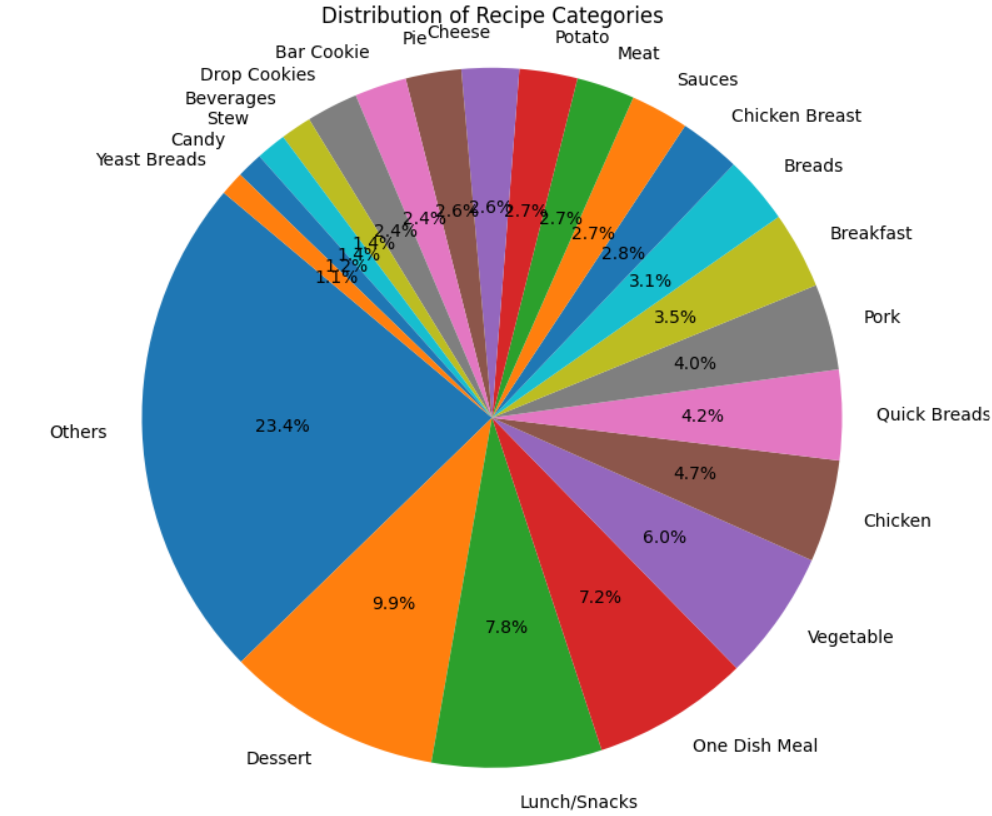
\includegraphics[width=0.4\textwidth]{1.png}
\caption{Distribution of Recipe Categories}
\label{fig:distribution_categories}
\end{figure}

\subsection{Distribution of All Ratings}

A count plot is used to visualize the distribution of all ratings. This plot provides an overview of the distribution of ratings assigned to recipes in the dataset.

\begin{figure}[H]
\centering
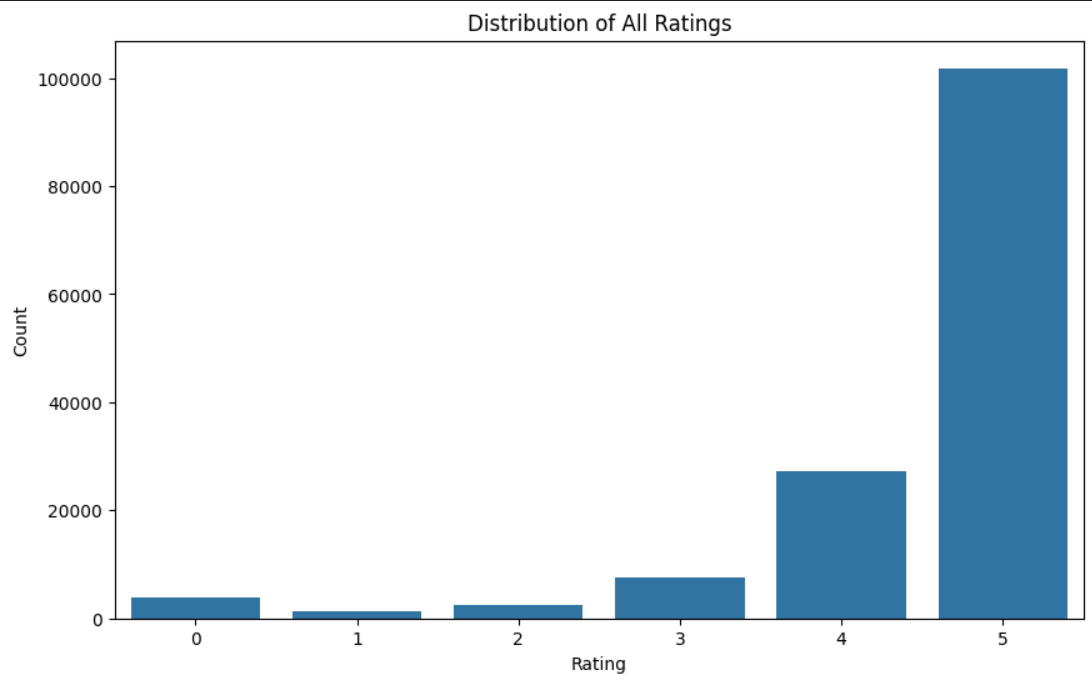
\includegraphics[width=0.4\textwidth]{2.png}
\caption{Distribution of All Ratings}
\label{fig:distribution_ratings}
\end{figure}


\subsection{Monthly Recipe Publication}

A line plot is utilized to illustrate the monthly publication of recipes over time. This visualization helps identify trends and patterns in recipe publication frequency.

\begin{figure}[H]
\centering
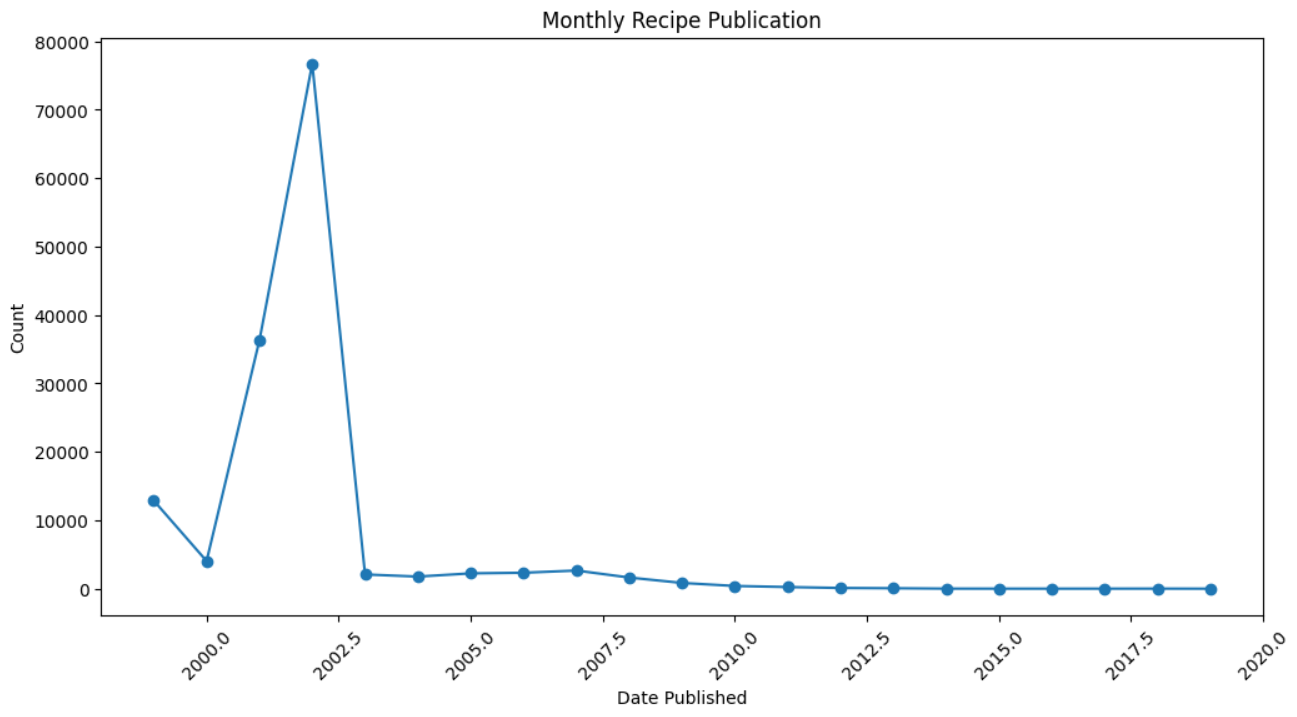
\includegraphics[width=0.4\textwidth]{3.png}
\caption{Monthly Recipe Publication}
\label{fig:monthly_publication}
\end{figure}

\subsection{Distribution of Calories}

The distribution of calories in recipes is displayed using a pie chart, categorizing calorie ranges into bins. This visualization offers insights into the distribution of calorie content across recipes.

\begin{figure}[H]
\centering
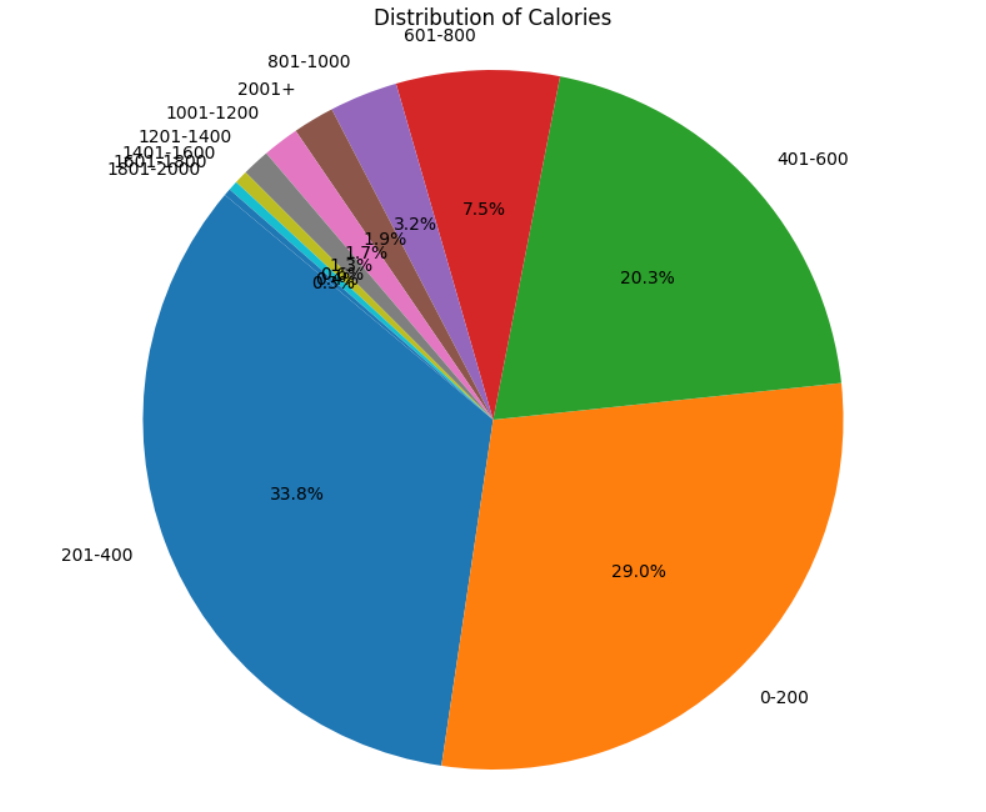
\includegraphics[width=0.4\textwidth]{4.png}
\caption{Distribution of Calories}
\label{fig:distribution_calories}
\end{figure}

\subsection{Top 10 Recipes by Review Count}

A bar plot is employed to showcase the top 10 recipes based on review count. This visualization highlights recipes that have received the highest number of reviews from users.

\begin{figure}[H]
\centering
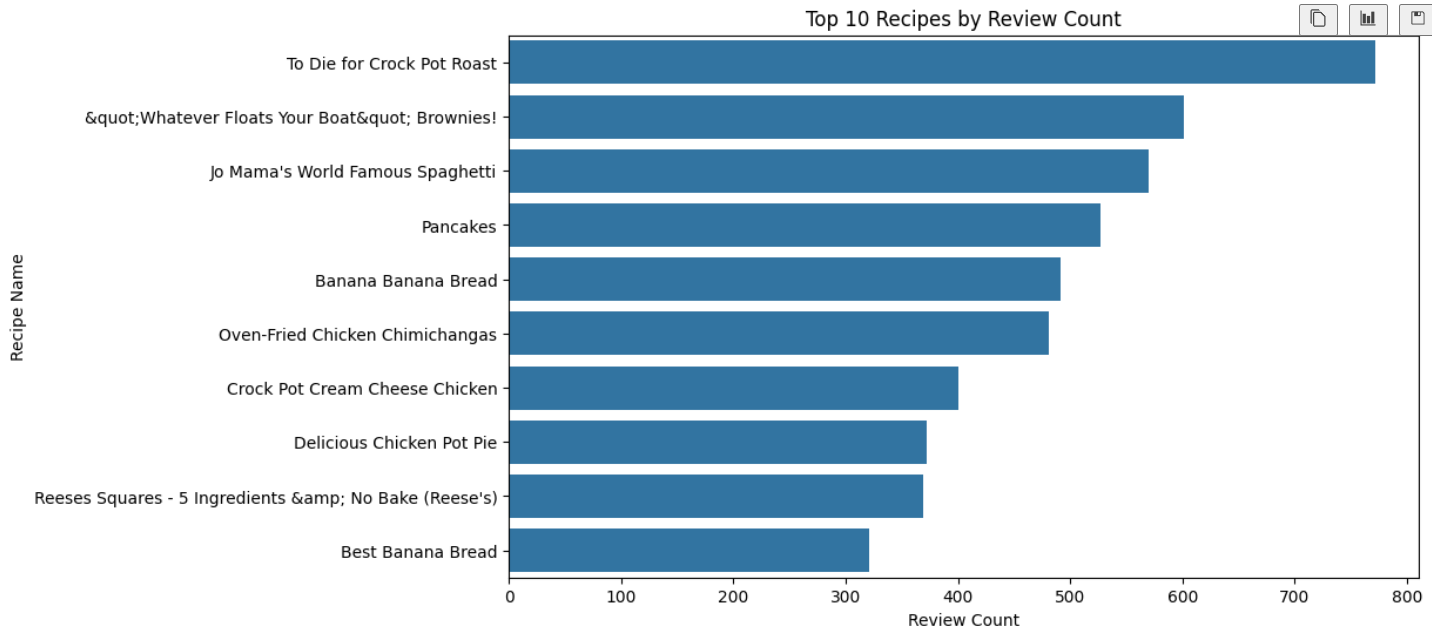
\includegraphics[width=0.4\textwidth]{5.png}
\caption{Top 10 Recipes by Review Count}
\label{fig:top10_recipes}
\end{figure}

\subsection{Top 10 Authors by Review Count}

Similarly, a bar plot is utilized to present the top 10 authors based on review count. This visualization identifies authors who have contributed the most reviewed recipes in the dataset.

\begin{figure}[H]
\centering
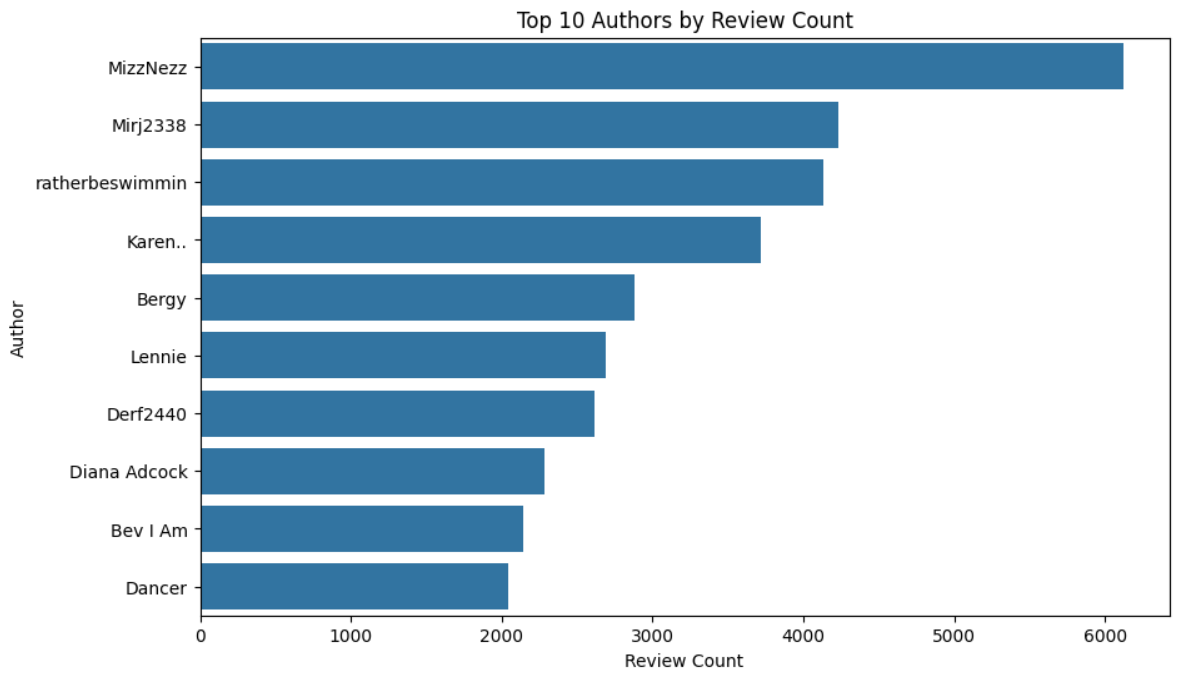
\includegraphics[width=0.4\textwidth]{6.png}
\caption{Top 10 Authors by Review Count}
\label{fig:top10_authors}
\end{figure}

Each visualization offers valuable insights into different aspects of the recipe dataset, aiding in understanding user preferences, recipe popularity, and publication trends.

\section{Content-Based Filtering}

Content-based filtering is a recommendation technique that suggests items to users based on their preferences and item features. In this section, we describe the implementation of content-based filtering for recipe recommendations using ingredient information.

\subsection{Extracting Unique Recipes}

First, unique recipes are extracted from the dataset to ensure that each recipe is considered only once for recommendation.

\subsection{TF-IDF Vectorization}

TF-IDF (Term Frequency-Inverse Document Frequency) vectorization is applied to the recipe ingredient parts to convert text data into numerical vectors. This process captures the importance of each ingredient in the recipe while considering its frequency across all recipes.

\subsection{Computing Cosine Similarity and Indexing}

Cosine similarity is calculated between the TF-IDF vectors of recipes to measure the similarity between them. An index is created to map recipe names to their corresponding indices in the dataset for efficient retrieval.

\subsection{Recommendation Function}

A recommendation function is defined to provide recommendations based on the similarity scores calculated using cosine similarity. Given a recipe title, the function returns a list of top recommended recipes with similar ingredient profiles.

\subsection{Printing Recommendations}

Recommendations are printed for sample recipe titles, such as 'Buttermilk Pie' and 'Potato Salad'. The function returns a list of recommended recipes based on the ingredient similarities with the input recipe.

---

Example Recommendations:

For the input recipe 'Buttermilk Pie', the following recommendations are provided:
\begin{itemize}
    \item Chocolate Dessert Crepes
    \item Easy Red Velvet Cake
    \item Red Velvet Waffles
    \item Filled Coffee Cake
    \item Peanut Butter Fudge Cake
\end{itemize}

For the input recipe 'Potato Salad', the following recommendations are provided:
\begin{itemize}
    \item Amish Potato Salad
    \item Mom's Danish Potato Salad
    \item Kathy's Macaroni Salad
    \item Curry Deviled Eggs With Cilantro
    \item Pickled Eggs
\end{itemize}

\section{Collaborative Filtering}

Collaborative filtering is a recommendation technique that identifies patterns in user behavior and preferences to recommend items to users. In this section, we describe the implementation of collaborative filtering for recipe recommendations using a reviewer-recipe-rating matrix.

\subsection{Creating Reviewer-Recipe-Rating Matrix}

A reviewer-recipe-rating matrix is constructed from the processed dataset, where each row represents a reviewer, each column represents a recipe, and the values represent the ratings given by reviewers to recipes. Missing ratings are filled with zeros.

\begin{table}[H]
\centering
\resizebox{\textwidth}{!}{%
\begin{tabular}{lcccccccccc}
\toprule
\textbf{ReviewerName} & \textbf{Recipe 1} & \textbf{Recipe 2} & \textbf{Recipe 3} & \textbf{Recipe 4} & \textbf{...} & \textbf{Recipe N} \\
\midrule
Reviewer 1 & 5 & 0 & 0 & 0 & ... & 4 \\
Reviewer 2 & 0 & 4 & 0 & 0 & ... & 0 \\
Reviewer 3 & 0 & 0 & 3 & 0 & ... & 0 \\
... & ... & ... & ... & ... & ... & ... \\
Reviewer M & 0 & 0 & 0 & 0 & ... & 2 \\
\bottomrule
\end{tabular}%
}
\caption{Reviewer-Recipe-Rating Matrix (excerpt)}
\label{tab:reviewer_recipe_matrix}
\end{table}

\subsection{Calculating Cosine Similarity Matrix}

Cosine similarity is computed between reviewers based on their rating vectors using the reviewer-recipe-rating matrix. This similarity matrix captures the similarity between pairs of reviewers, indicating how alike their preferences are.

\begin{table}[H]
\centering
\resizebox{\textwidth}{!}{%
\begin{tabular}{lcccccc}
\toprule
\textbf{ReviewerName} & \textbf{Reviewer 1} & \textbf{Reviewer 2} & \textbf{Reviewer 3} & \textbf{...} & \textbf{Reviewer M} \\
\midrule
Reviewer 1 & 1.0 & 0.8 & 0.6 & ... & 0.4 \\
Reviewer 2 & 0.8 & 1.0 & 0.7 & ... & 0.5 \\
Reviewer 3 & 0.6 & 0.7 & 1.0 & ... & 0.3 \\
... & ... & ... & ... & ... & ... \\
Reviewer M & 0.4 & 0.5 & 0.3 & ... & 1.0 \\
\bottomrule
\end{tabular}%
}
\caption{Cosine Similarity Matrix (excerpt)}
\label{tab:cosine_similarity_matrix}
\end{table}

\subsection{Predicting Ratings for Missing Entries}

Predictions for missing ratings for each user are made one by one. This involves identifying similar users and using their ratings for the target recipe to predict missing rating. The predictions are based on the cosine similarity scores between users. 
\\
It is used to in a way assign optimum weights to each other reviewer's rating. The users having rating vector similar to target user will have higher weight and vice versa. Weighted sum of these ratings is taken to predict target user's rating for the recipe.

---

Please note that the full matrices may be too large to display in their entirety. Only excerpts are shown here for illustration purposes.

% Individual Contribution
\section{Individual Contributions}
\subsection{Himang Chandra Garg}
\begin{itemize}
    \item Implemented data visualization techniques using Matplotlib and Seaborn libraries.
    \item Developed the content-based filtering algorithm using TF-IDF vectorization and cosine similarity.
\end{itemize}

\subsection{Nishil Agarwal}
\begin{itemize}
    \item Implemented data preprocessing pipeline, including filtering, cleaning, and formatting of the dataset.
    \item Developed the collaborative filtering algorithm for generating user-based recommendations.
\end{itemize}

% References
\begin{thebibliography}{99}
\bibitem{reference1}
https://www.kaggle.com/datasets/irkaal/foodcom-recipes-and-reviews

\end{thebibliography}


\end{document}
